\documentclass[table]{beamer}
\mode<presentation>
{
    \usetheme[backgroundimagefile=images/background.jpg]{diepen}
    \usefonttheme{structurebold}
}

\usepackage[english]{babel}
\usepackage[utf8x]{inputenc}
\usepackage[T1]{fontenc}
\usepackage{graphicx}
\usepackage{tabularx}
\usepackage{amsmath}
\usepackage{amssymb}
\usepackage{xcolor,soul}
\usepackage{tikz}
\usepackage{minted}
\usepackage{MnSymbol}
\usepackage{datetime}
\usepackage{hyperref}
\usepackage{tabu}
\usepackage{multirow}
\usepackage{tikz}
\usepackage{wrapfig}
\usepackage[small]{caption}
\usepackage[version-1-compatibility]{siunitx}
\DeclareGraphicsExtensions{.pdf, .jpg, .tif, .eps, .png}
\graphicspath{{images/}{images/pdf/}{images/png}{images/jpg/}}
\hypersetup{colorlinks=true, linkcolor=black}

\newcommand{\pitem}{\pause \item}

\let\oldsqrt\sqrt
\def\sqrt{\mathpalette\DHLhksqrt}
\def\DHLhksqrt#1#2{%
\setbox0=\hbox{$#1\oldsqrt{#2\,}$}\dimen0=\ht0
\advance\dimen0-0.2\ht0
\setbox2=\hbox{\vrule height\ht0 depth -\dimen0}%
{\box0\lower0.4pt\box2}}

\makeatletter
\newsavebox\myboxA
\newsavebox\myboxB
\newlength\mylenA
\newcommand*\xbar[2][0.75]{%
    \sbox{\myboxA}{$\m@th#2$}%
    \setbox\myboxB\null% Phantom box
    \ht\myboxB=\ht\myboxA%
    \dp\myboxB=\dp\myboxA%
    \wd\myboxB=#1\wd\myboxA% Scale phantom
    \sbox\myboxB{$\m@th\overline{\copy\myboxB}$}%  Overlined phantom
    \setlength\mylenA{\the\wd\myboxA}%   calc width diff
    \addtolength\mylenA{-\the\wd\myboxB}%
    \ifdim\wd\myboxB<\wd\myboxA%
       \rlap{\hskip 0.5\mylenA\usebox\myboxB}{\usebox\myboxA}%
    \else
        \hskip -0.5\mylenA\rlap{\usebox\myboxA}{\hskip 0.5\mylenA\usebox\myboxB}%
    \fi}
\makeatother
% vim: set filetype=tex:


\title{Aerial Photogrammetry for Volcanology} % Title under consideration
\author{Drew Silcock}
\institute{University of Bristol, Department of Earth Sciences}
\longdate{}

\begin{document}

\begin{frame}
    \titlepage
\end{frame}

\begin{frame}{Outline}
    \tableofcontents
\end{frame}

\section{Introduction}

\subsection{Photogrammetry}

\begin{frame}{What Is Photogrammetry?}
    \begin{itemize}
        \item Also known as \textit{structure from motion}
        \item Parallax from photos taken from different positions
        \item Reconstruct 3D model of object
        \item No need to know camera positions! (although it helps...)
        \item Used by Google for Google Earth
        \item Building Rome in a day (150,000 Flickr images, 496 cores, 21
            hours):
    \end{itemize}
    \begin{center}
        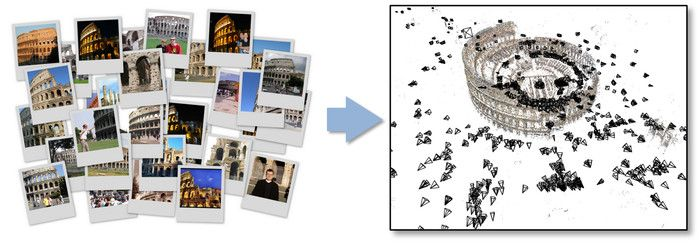
\includegraphics[width=0.75\linewidth]{Colosseum}
    \end{center}
\end{frame}

\subsection{Photo Taking Technique}

\begin{frame}{Taking Photos}
    \begin{center}
        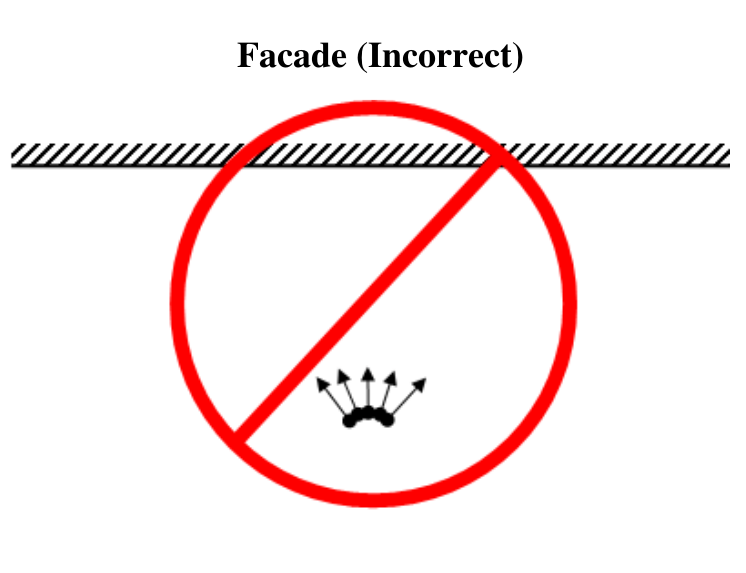
\includegraphics[width=0.7\paperwidth]{Incorrect}
    \end{center}
\end{frame}

\begin{frame}{Taking Photos}
    \begin{center}
        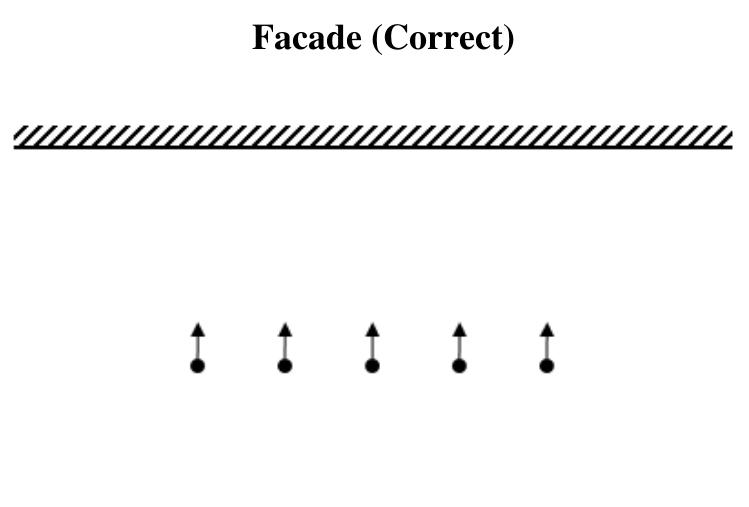
\includegraphics[width=0.8\paperwidth]{Correct}
    \end{center}
\end{frame}

\section{Software Used}

\subsection{Agisoft PhotoScan}

\begin{frame}{Agisoft Photoscan}
    \begin{itemize}
        \item Input photos of an object from different positions
        \item Uses parallax to generate sparse point cloud
        \item Uses sparse point cloud to generate dense point cloud
        \item Uses dense point cloud to generates mesh (connect the dots)
        \item Overlaps texture from photos on top (texture)
    \end{itemize}
\end{frame}

\begin{frame}{Agisoft Photoscan}
    Here's what it looks like in action:
    \begin{center}
        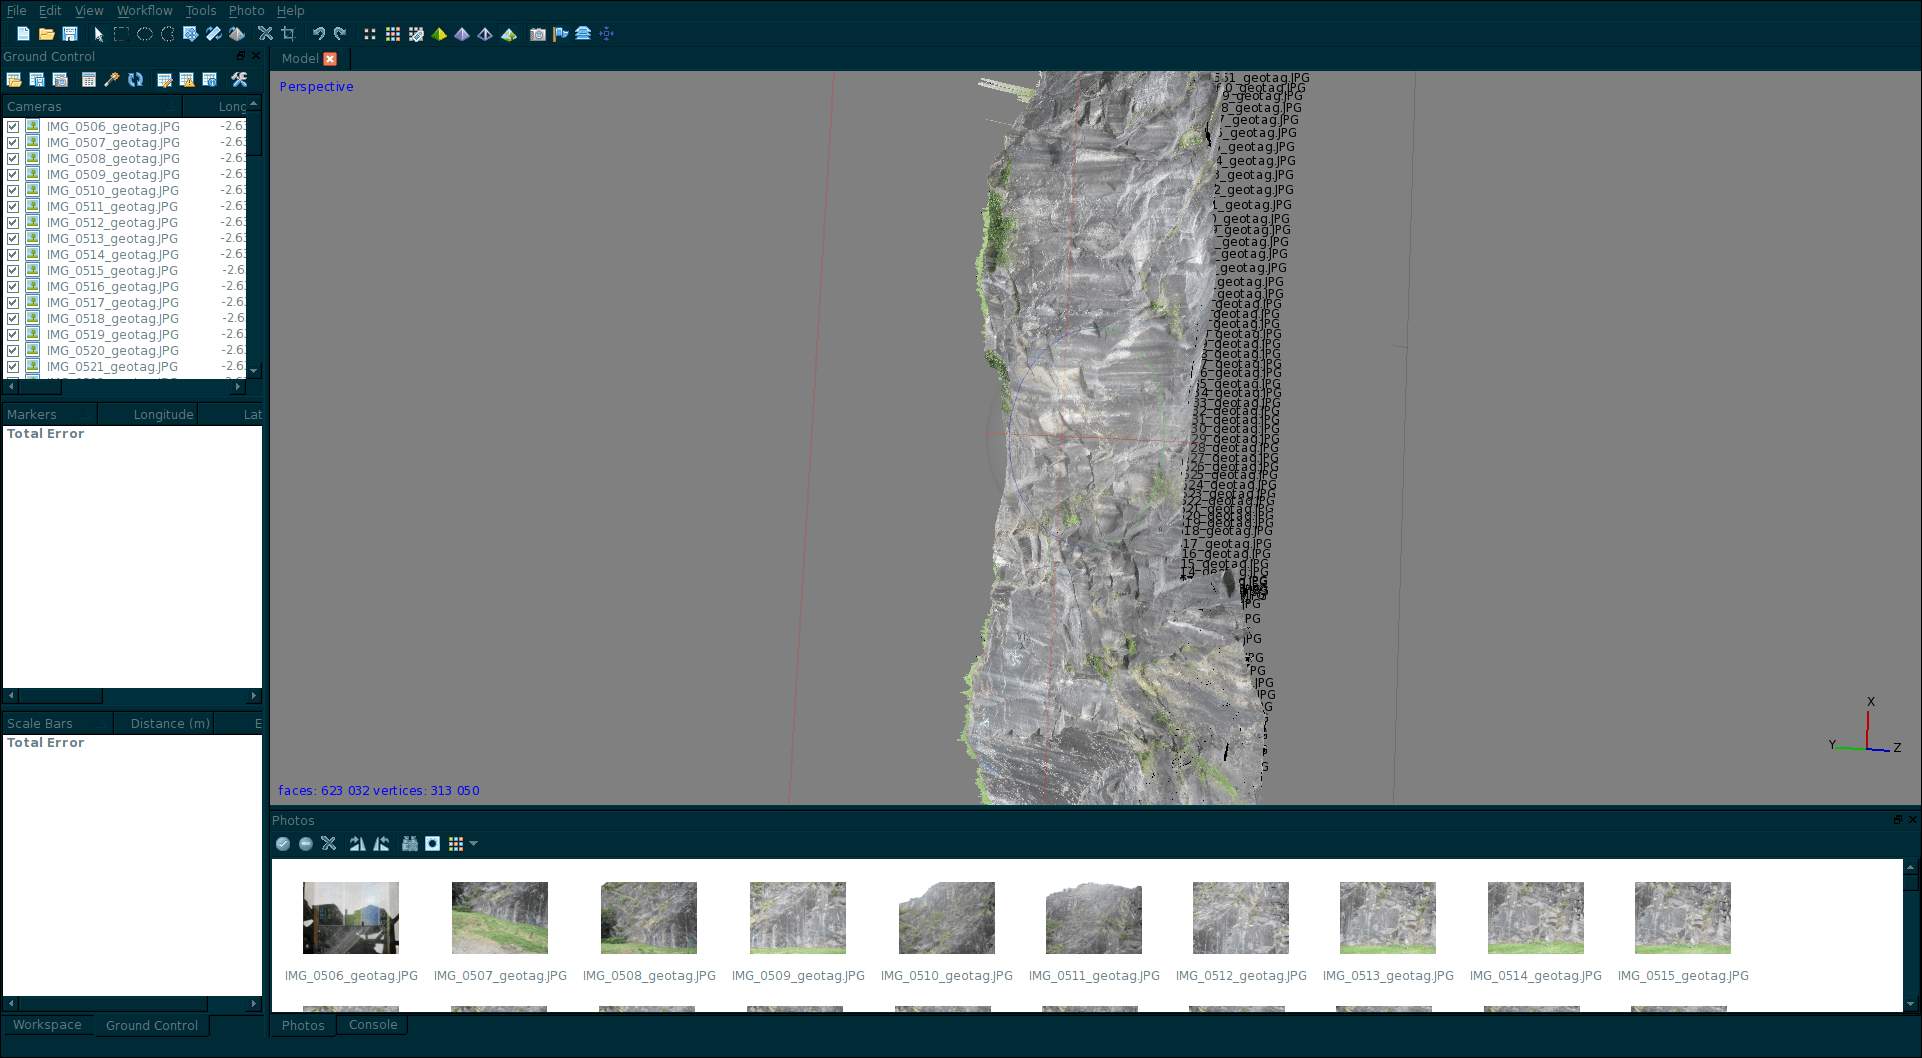
\includegraphics[width=\linewidth]{PhotoScan}
    \end{center}
\end{frame}

\begin{frame}{Agisoft Photoscan}
    Here's what it produces:
    \begin{center}
        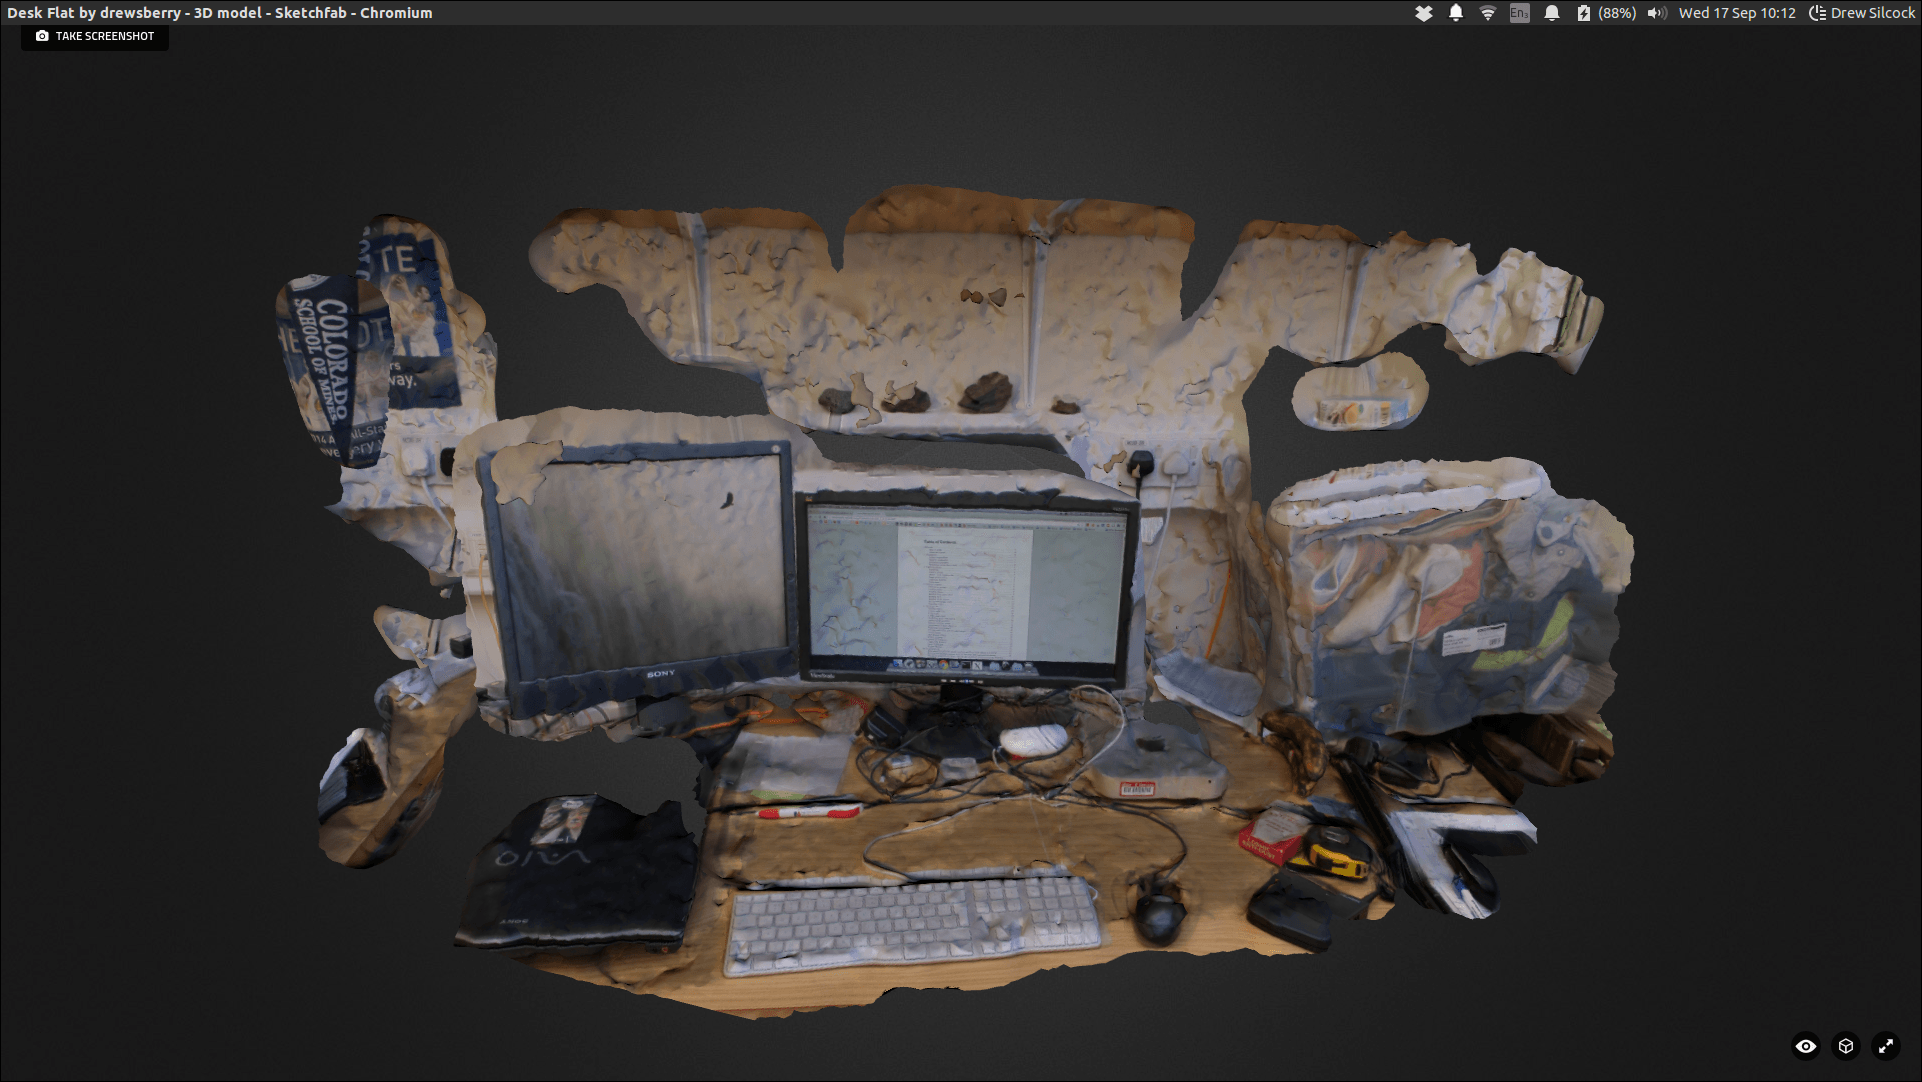
\includegraphics[width=\linewidth]{MyDesk}
    \end{center}
\end{frame}

\subsection{Mission Planner and APM}

\begin{frame}{Mission Planner and APM}
    \begin{columns}[T]
        \begin{column}[T]{5cm}
            \begin{itemize}
                \item ArduPilot Mega (APM): autopilot for UAV
                \item Takes instruction from Mission Planner (MP)
                \item MP can:
                    \begin{enumerate}
                        \item Set waypoints for UAV
                        \item Tell UAV to hover
                        \item Tell UAV to take photos (theoretically)
                        \item Geotag photos from log or time offset (more on
                            this later)
                    \end{enumerate}
            \end{itemize}
        \end{column}
        \begin{column}[T]{7cm}
            \begin{center}
                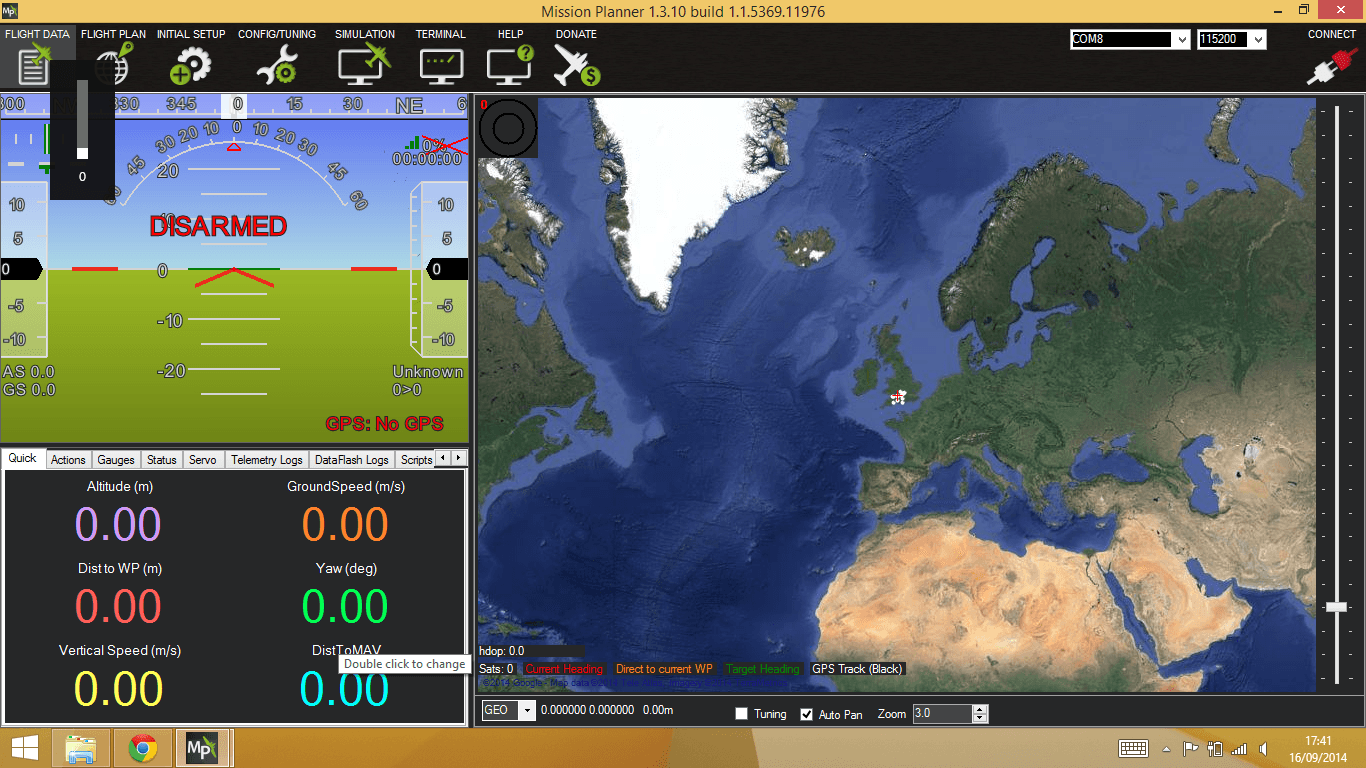
\includegraphics[width=\columnwidth]{MissionPlanner}
            \end{center}
        \end{column}
    \end{columns}
\end{frame}

\subsection{Canon Hack Development Kit}

\begin{frame}{Canon Hack Development Kit}
    \begin{itemize}
        \item Pretty cool hack for Canon cameras
        \item Allows you to set camera to take pictures every 5 seconds, take
            photos on electronic input, etc.
        \item Executes scripts written in Lua or UBASIC
    \end{itemize}
    \begin{center}
        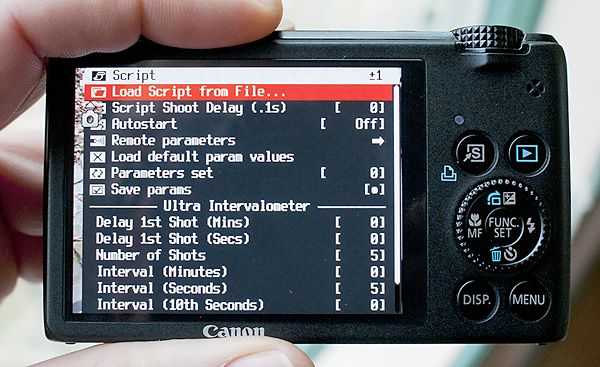
\includegraphics[width=0.6\columnwidth]{CHDKDisplay}
    \end{center}
\end{frame}

\section{Uses}

\subsection{Lava Flow}

\begin{frame}{Uses}
    \begin{itemize}
        \item As with Lidar (see Oscar's presentation)
        \item Studying lava flow
        \item Lava flow prediction
        \item UAVs able to get where traditionally it was not possible
        \item Cheap (buy simply point and shoot from Amazon)
        \item Light (especially useful for putting on UAVs)
    \end{itemize}
\end{frame}

\section{Metholodogy}

\begin{frame}{Taking Photos}
    Two options:
    \begin{description}
        \item[Time delay] Tell CHDK to take pictures every 5 seconds, strap it onto your UAV
            and you're ready to go
        \item[CAM messages] Tell CHDK to take photos whenever it receives an electronic signal
            of a particular kind (Pulse Width Modulation). APM then logs this
            event.
    \end{description}
    Latter is better for geotagging (next slide), but also a huge pain to get to
    work...
\end{frame}

\subsection{Geotagging}

\begin{frame}{Geotagging - Time Delay}
    \begin{itemize}
        \item APM keeps a log of GPS location, time, yaw and roll
        \item Tell MP offset between first photo and first log message (take
            picture of screen), give it log and photos and it geotags them
        \item Two types of logs:
            \begin{description}
                \item[Telemetry logs (\texttt{.tlog})] \hfill \\
                    Taken while MP connected to APM by USB and saved to MP
                    computer
                \item[Dataflash logs (\texttt{.log})] \hfill \\
                    Taken while the copter is armed and saved to APM flash
                    storage; download later when connected to MP
            \end{description}
        \item Dataflash used when aerial
    \end{itemize}
\end{frame}

\begin{frame}{Geotagging - CAM Messages}
    \begin{columns}[T]
        \begin{column}[T]{5cm}
            \begin{itemize}
                \item APM tells CHDK to shoot
                \item APM logs CAM message: time, location, roll and yaw
            \end{itemize}
        \end{column}
        \begin{column}[T]{5cm}
            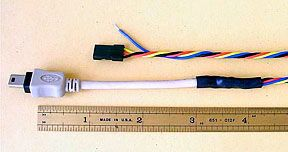
\includegraphics[width=\textwidth]{CHDKCable}
        \end{column}
    \end{columns}
    \begin{itemize}
        \item CAM log message specified by: \\
            {\scriptsize\texttt{FMT,~18,~27,~CAM,~IHLLeccC,~GPSTime,GPSWeek,Lat,Lng,Alt,Roll,Pitch,Yaw}}
        \item So look out for something in your log that looks like: \\
            {\scriptsize\texttt{CAM,~57263726,~1790,~54.4136582,~-3.5039962,~62.74,~7.12,~8.56,~12.01}}
        \item Give MP your photos and your \texttt{.log}, and it
            automatically geotags them for you
    \end{itemize}
\end{frame}

\subsection{Ground Control Points}

\begin{frame}{Ground Control Points}
    \begin{itemize}
        \item To help with the photogrammetric reconstruction, we employ GCPs
        \item Measure in the exact location of a coordinate, marked with a
            distinguishable feature (e.g. cross)
        \item Tell PhotoScan where that mark is geographically as co-ordinates
            in local reference or WGS 84
        \item PhotoScan optimises point cloud generation
        \item Improved accuracy and precision
    \end{itemize}
\end{frame}

\begin{frame}{Ground Control Points}
    \begin{center}
        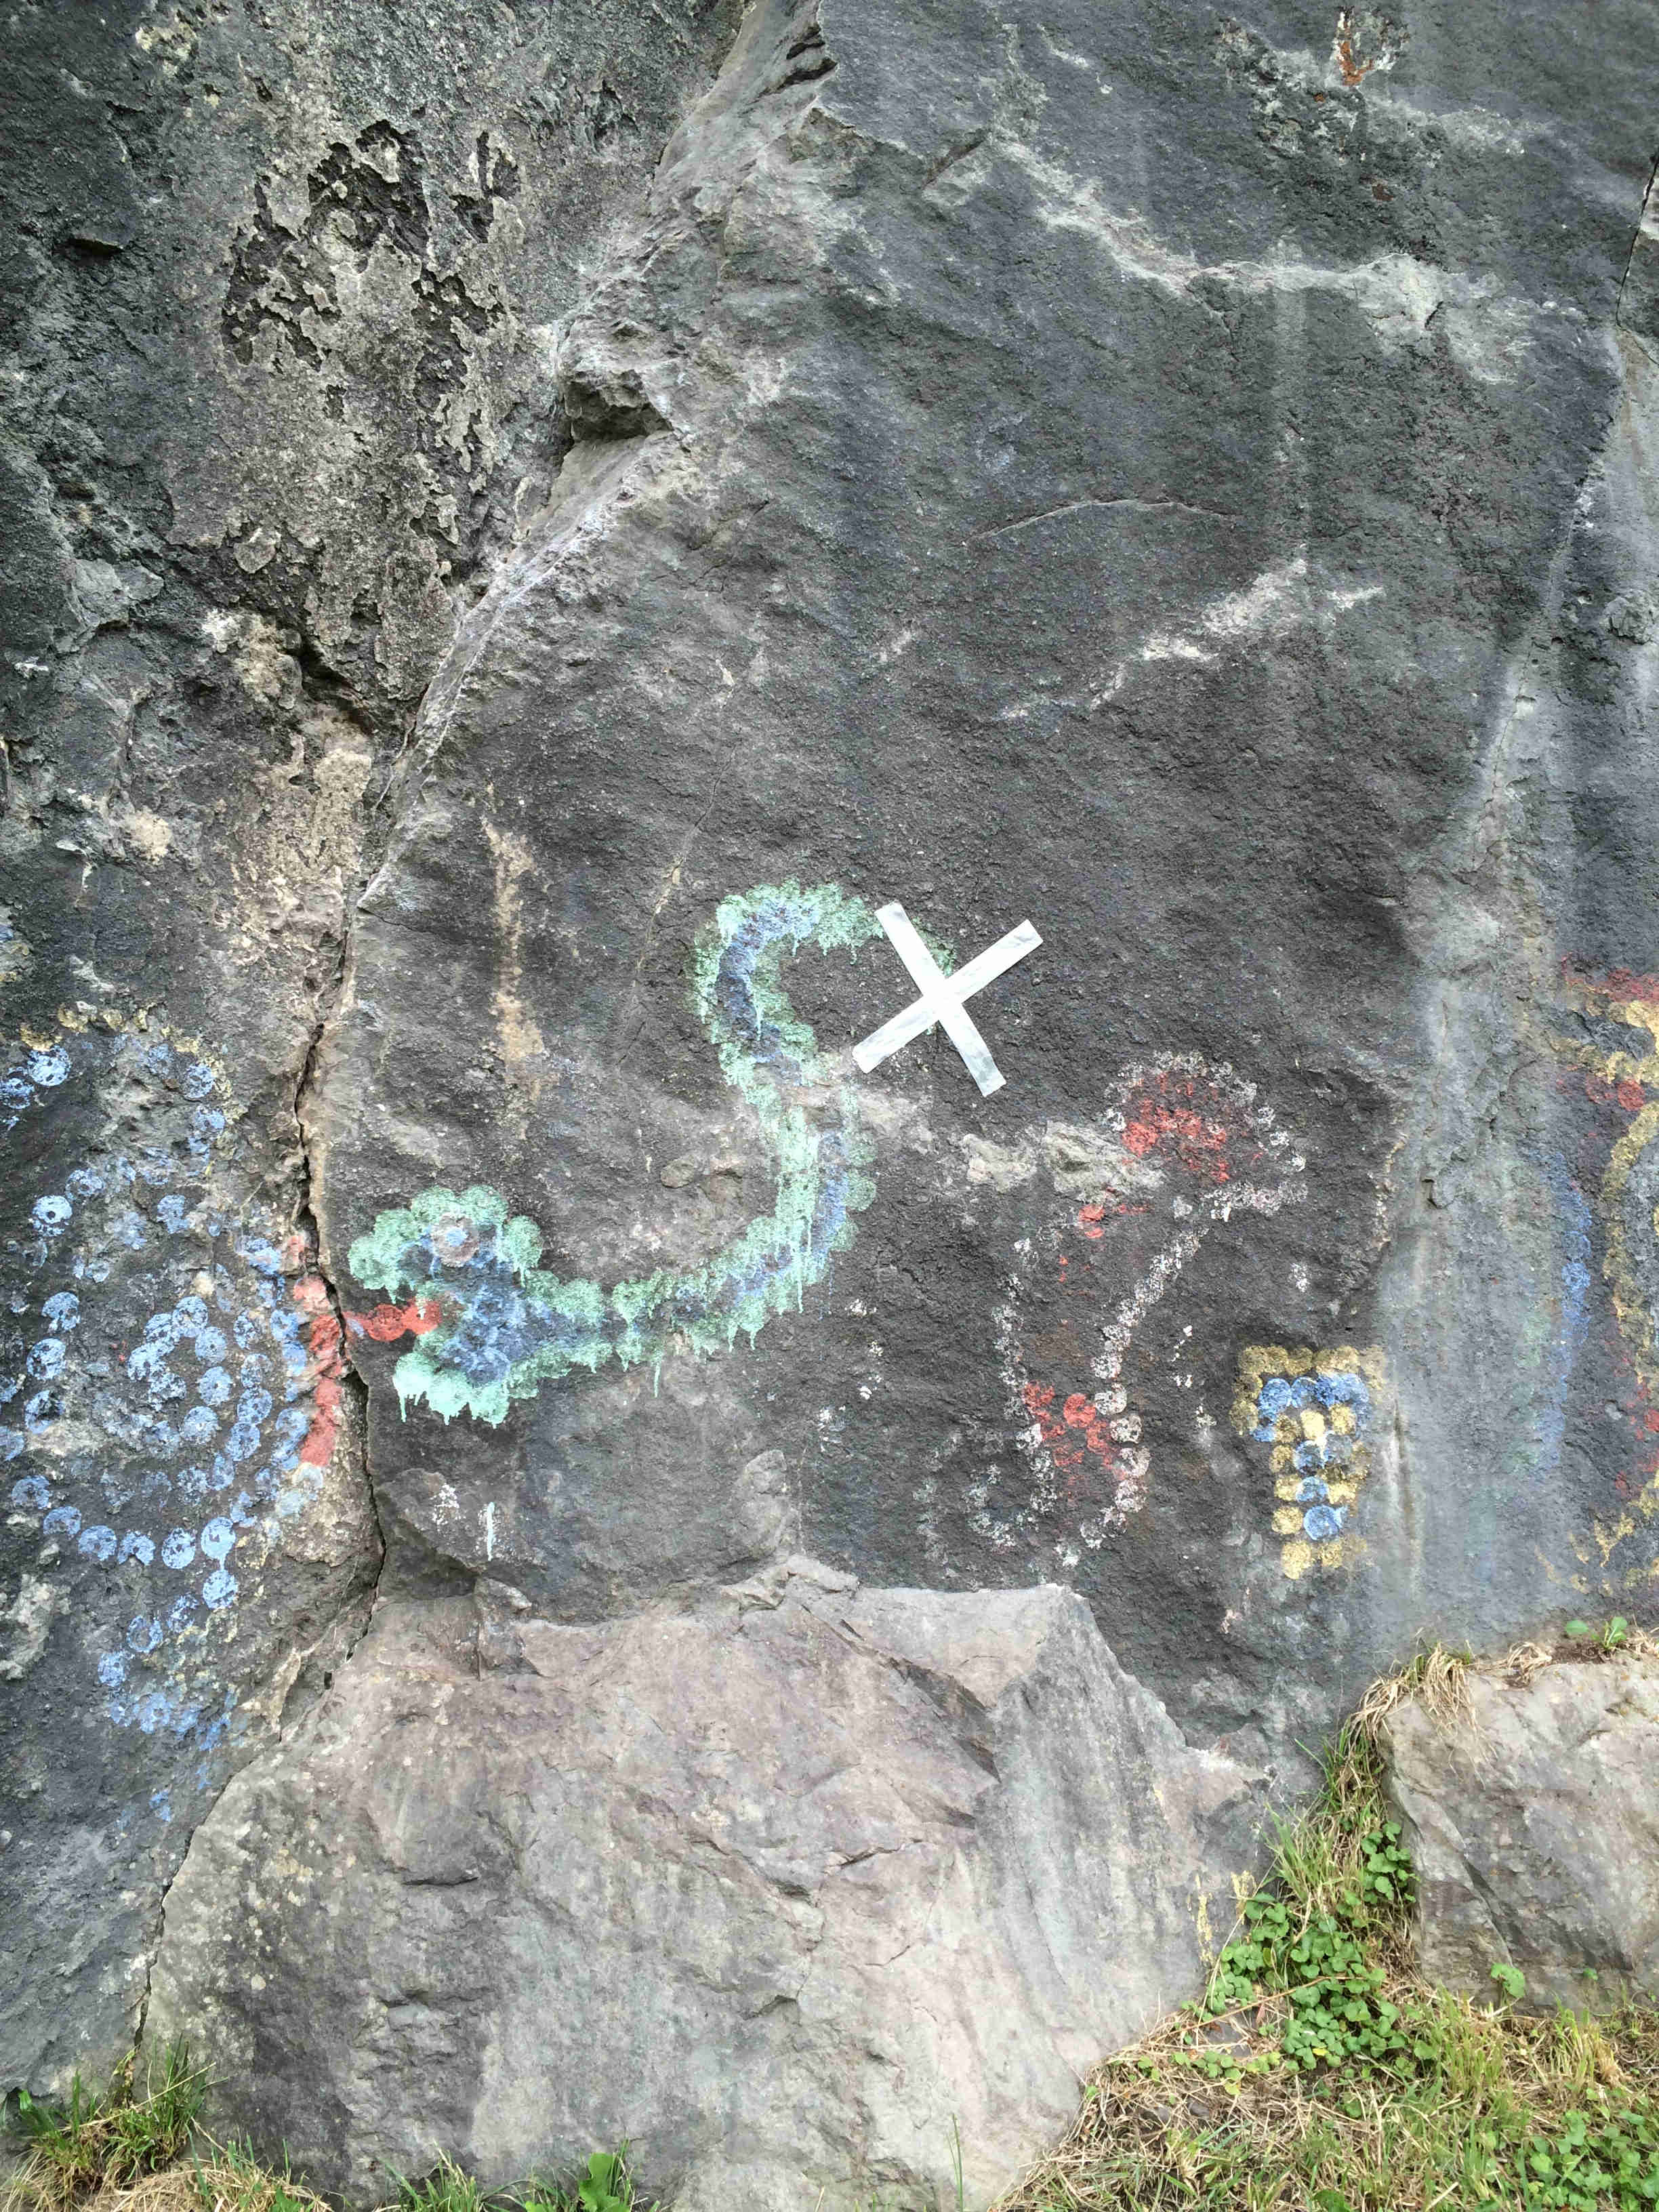
\includegraphics[width=0.45\linewidth]{GCP} ~
        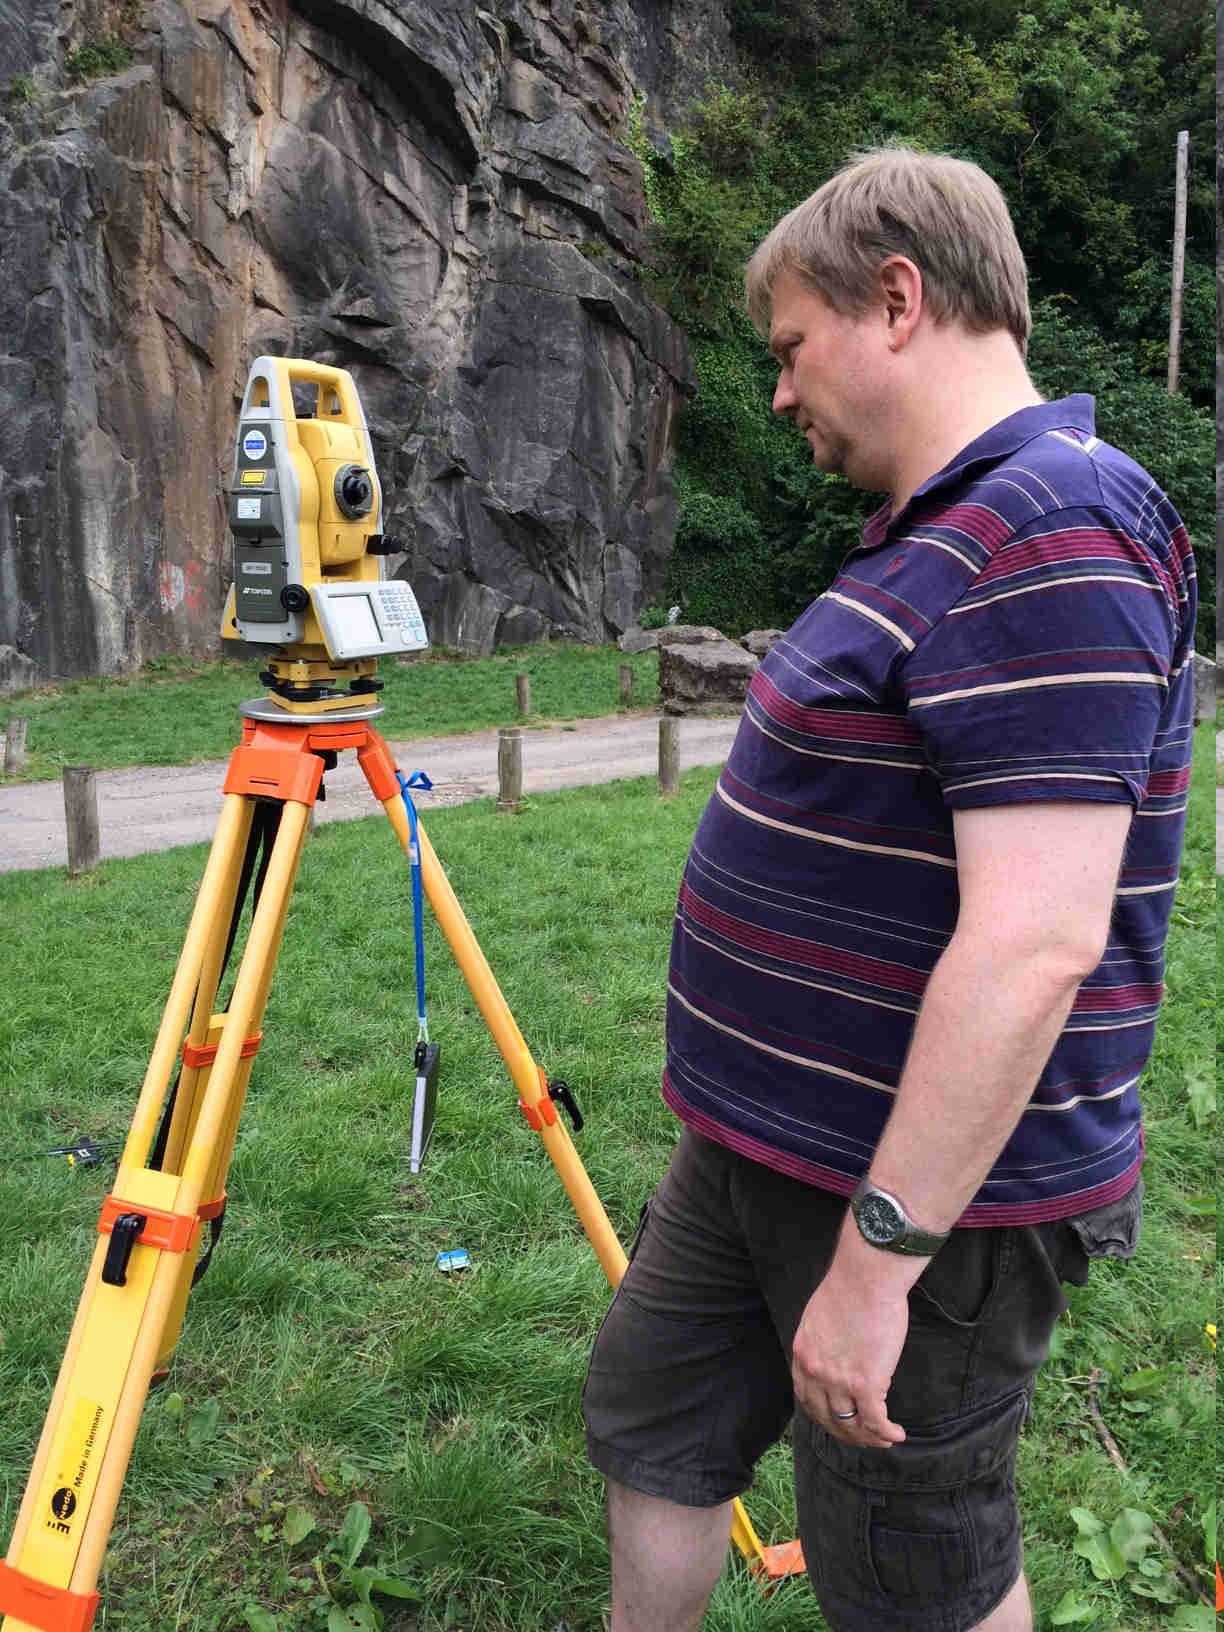
\includegraphics[width=0.45\linewidth]{GCPEquipment}
    \end{center}
\end{frame}

\subsection{Accuracy and Precision}

\begin{frame}{Accuracy and Precision}
    \begin{itemize}
        \item Meters per pixel as function of height
        \item Minimum UAV speed needed to give required overlap (80\%)
        \item Agisoft generated reports give m/pix, error in pix, DEM error in
            pix
    \end{itemize}
    \begin{center}
        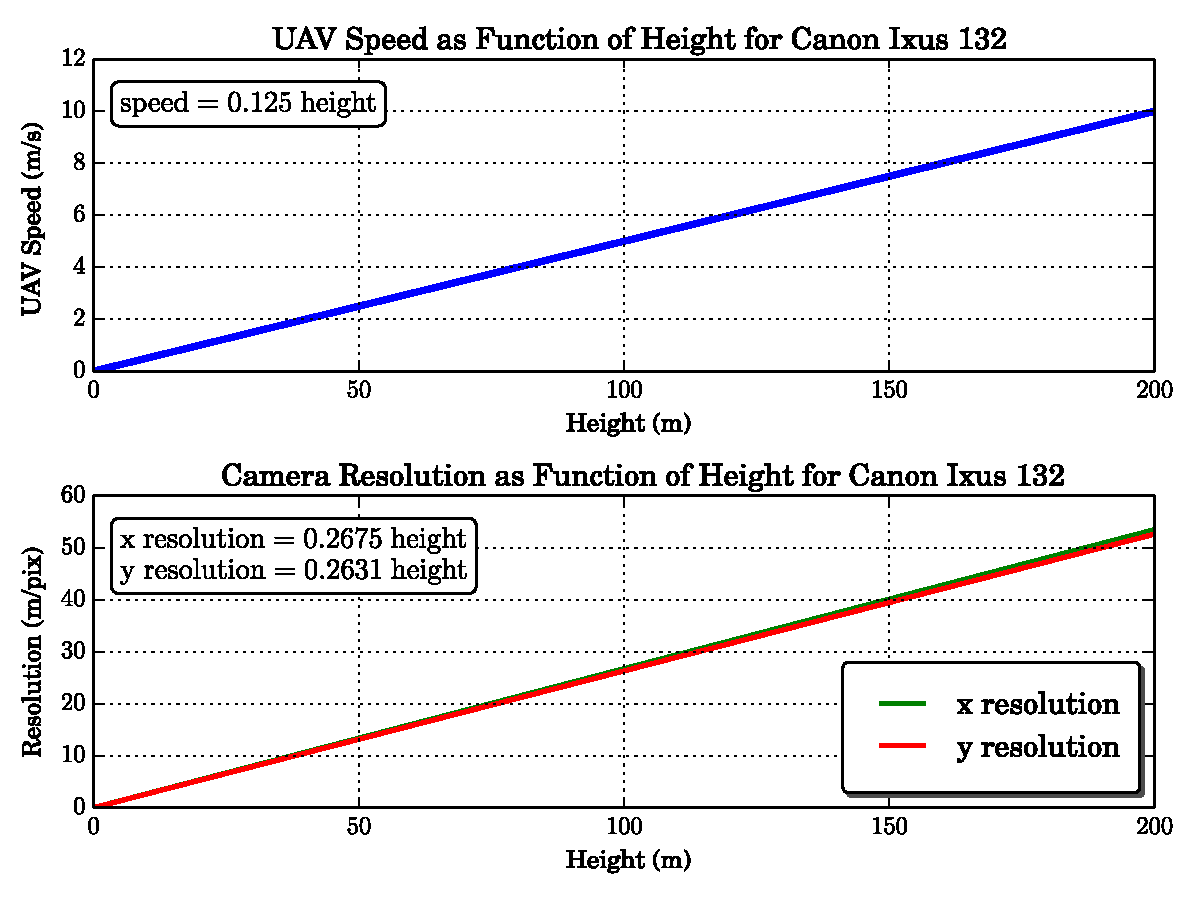
\includegraphics[width=0.6\linewidth]{HeightPlots}
    \end{center}
\end{frame}

\section{Results}

\begin{frame}{Results}
    \begin{description}
        \item[Aerial Survey] \hfill \\
            \begin{itemize}
                \item Long Ashton field
                \item Partly mapped, before everything broke
                \item PhotoScan generated DEM, orthophoto, photo overlap, GCP
                    data and accuracy
            \end{itemize}
        \item[Avon Gorge] \hfill \\
            \begin{itemize}
                \item Avon Gorge, big rock with cool fractures
                \item Horizontal instead of vertical
                \item PhotoScan generated DEM, orthophoto, photo overlap and accuracy
            \end{itemize}
    \end{description}
\end{frame}

\subsection{Aerial Survey}

\begin{frame}{Aerial Survey Without GCPs}
    \begin{center}
        \url{https://sketchfab.com/models/ec777be4b73f4e7a8fdd992c2b8d026a}
        \includegraphics[width=0.3\linewidth]{AerialSurveyOrthophoto}
        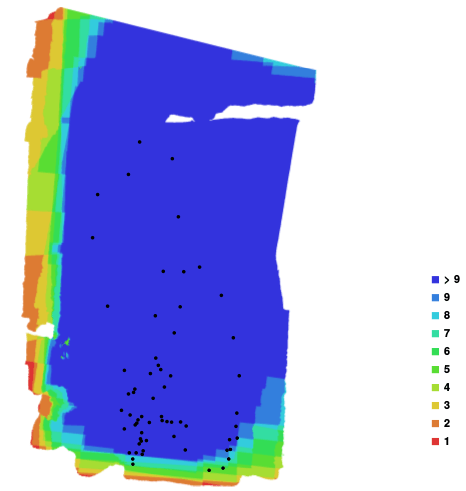
\includegraphics[width=0.3\linewidth]{AerialSurveyOverlap}
        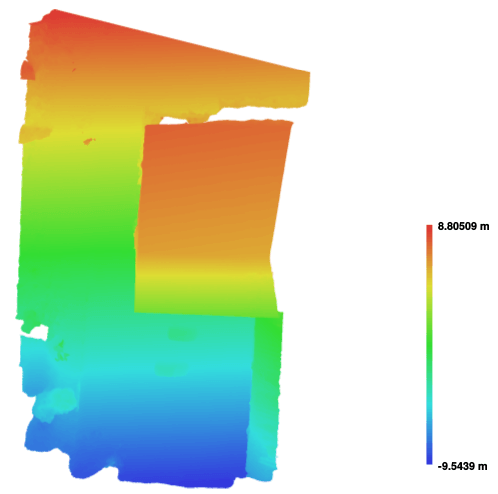
\includegraphics[width=0.3\linewidth]{AerialSurveyDEM}
    \end{center}
    \begin{center}
        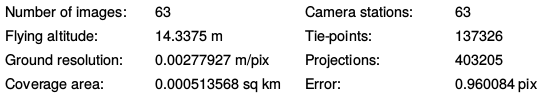
\includegraphics[width=\linewidth]{AerialSurveyAccuracy}
    \end{center}
\end{frame}

\begin{frame}{Aerial Survey With GCPs}
    \begin{center}
        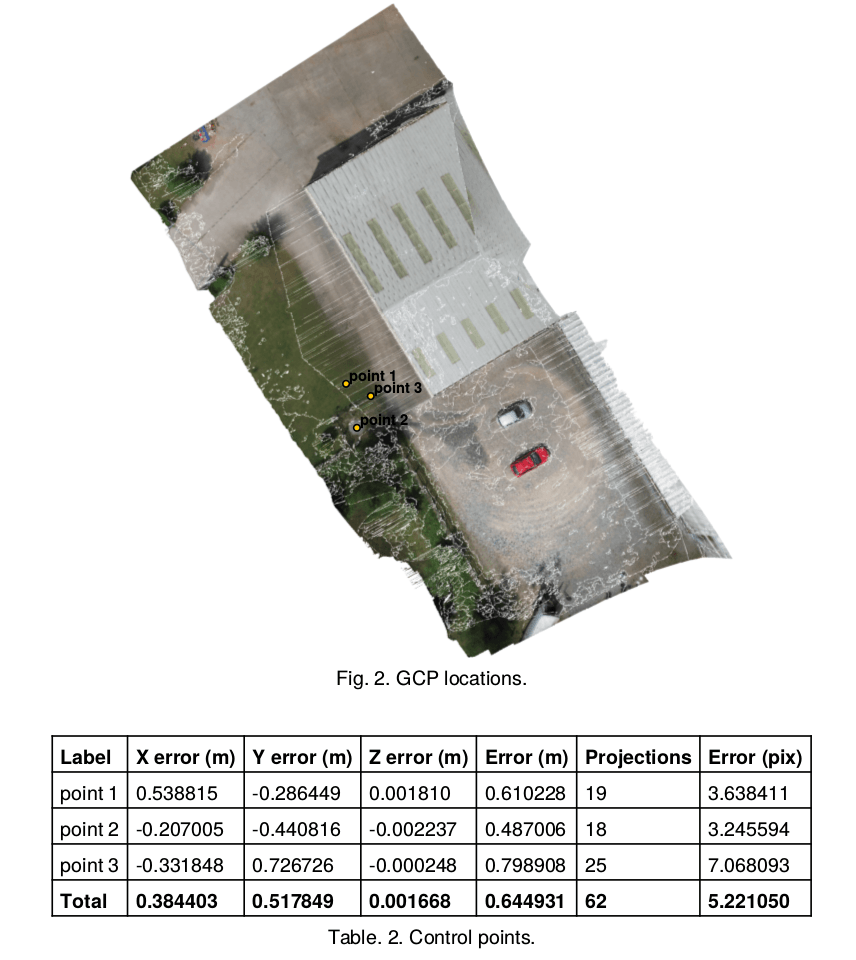
\includegraphics[width=0.45\linewidth]{AerialSurveyGCPs}
        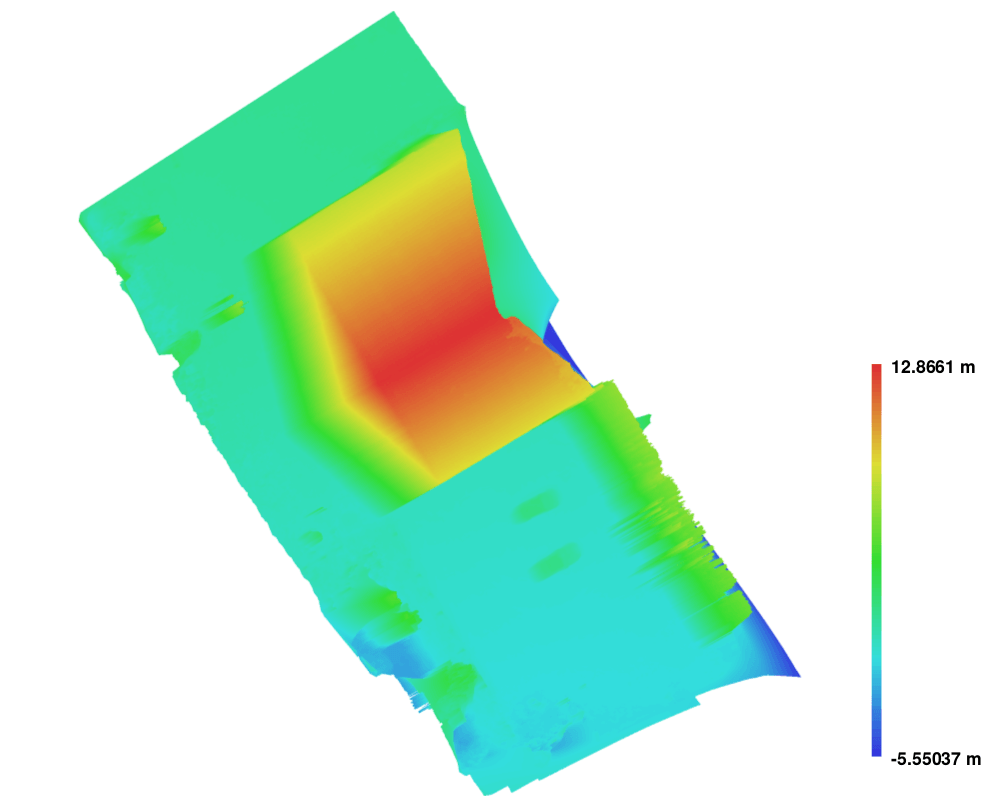
\includegraphics[width=0.45\linewidth]{AerialSurveyGCPsDEM}
    \end{center}
\end{frame}

\subsection{Avon Gorge}

\begin{frame}{Avon Gorge}
    \url{https://sketchfab.com/models/ad8a1d9f8c324eb592a9e4beabc5a51e}
    \begin{center}
        
\includegraphics[width=\linewidth]{AvonGorgeOrthophoto}
    \end{center}
    \begin{center}
        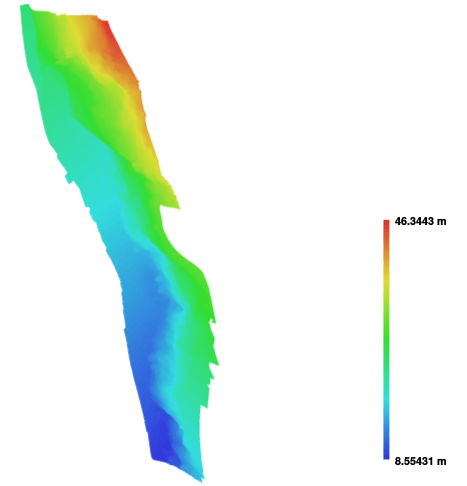
\includegraphics[width=0.3\linewidth]{AvonGorgeDEM}
        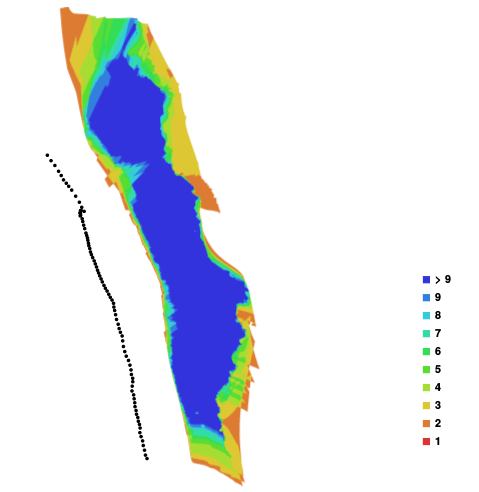
\includegraphics[width=0.3\linewidth]{AvonGorgeOverlap}
    \end{center}
\end{frame}

\section{Future Projects}

\begin{frame}{Future Projects}
    \begin{itemize}
        \item Figure out how to get MP to tell CHDK to take photos at waypoints
        \item Investigate more possible uses for Earth Science/Volcanology
        \item Write manual for future UAV/photogrammetry researcher
        \item Rerun reconstruction of Avon Gorge with GCPs
    \end{itemize}
\end{frame}

\begin{frame}{Lidar vs. Photogrammetry}
    \begin{columns}[c]
        \begin{column}[c]{5cm}
            \textbf{Pros of Photogrammetry}
            \begin{itemize}
                \item Cheap (doesn't matter if you drop it in some lava)
                \item Light (good for putting on UAVs)
            \end{itemize}
        \end{column}
        \begin{column}[c]{5cm}
            \textbf{Pros of Lidar}
            \begin{itemize}
                \item Very accurate and precise
                \item Real-time measurements - can make measurements of
                    dynamic, moving objects
            \end{itemize}
        \end{column}
    \end{columns}
\end{frame}

\end{document}
